

\documentclass[aos]{imsart}

\usepackage{type1cm}
\usepackage{titlesec}
\usepackage{float}
\RequirePackage{amsthm,amsmath,amsfonts,amssymb}
\RequirePackage[numbers]{natbib}
\RequirePackage{graphicx}


\newcommand{\cic}{\text{CIC}}
\newcommand{\cicFull}{\text{Cheskidov Correlation}}
\newcommand{\pcc}{\text{PCC}}
\newcommand{\pccFull}{\text{Pierson Correlation}}

\newcommand{\addExample}[8]{
  \begin{figure}[H]
\titleformat{\subsection}[hang]
  {\normalfont\fontsize{11pt}{13pt}\itshape}
  {\thesubsection}{1em} 
  {\makebox[0.6\textwidth][l]}

  \subsection{Example #1. #2}

\begin{minipage}[t]{0.45\textwidth}
    \vspace{0pt}
    \centering
    \resizebox{!}{4cm}{\includegraphics{#3}}
    \caption{#2)}
\end{minipage}
\hfill
\begin{minipage}[t]{0.50\textwidth}
    \vspace{20pt}

    \noindent
    $x = #4$ \\[4pt]
    $y(x) = #5$ \\[6pt]
    $\cic$ = $#6$, $\pcc$ = $#7$

    \medskip

    #8
\end{minipage}

\end{figure}
}


\startlocaldefs


\endlocaldefs

\begin{document}

\begin{frontmatter}

\title{Cheskidov Increment Correlation}

\runtitle{Cheskidov Correlation}


\begin{aug}

\author[A]{\fnms{Roman}~\snm{Cheskidov}\ead[label=e1]{t3531350@yahoo.com}},
\author[B]{\fnms{Alena}~\snm{Cheskidova}\ead[label=e2]{alyona.cheskidova@gmail.com}}

\address[A]{Independent Researcher, San Francisco, USA\printead[presep={,\ }]{e1}}
\address[B]{Ural Federal University, Yekaterinburg, RF\printead[presep={,\ }]{e2}}
\end{aug}

\begin{abstract}
The article introduces the Increment-Based Concordance Correlation Coefficient (Cheskidovs’) — Increment-based $\cic$ or $\cic$ — as a unit-free, consistent measure of synchrony that overcomes Pearson’s limitations in nonlinear and oscillatory data. By focusing on mutual increments, $\cic$ matches Pearson in monotonic cases but avoids false correlations in complex contexts, making it especially suited for ordered time-series such as financial or climate data. It reliably identifies true dependencies while remaining stable near zero for oscillatory patterns, offering a robust, complementary tool for modern data analysis where directionality of change is crucial.
\end{abstract}

\begin{keyword}[class=MSC]
\kwd[Primary ]{62H20}
\kwd[; Secondary ]{62M20, 62M10, 62R10, 62P05, 62P10, 62P20}
\end{keyword}

\begin{keyword}
\kwd{correlation coefficient}
\kwd{increment analysis}
\kwd{time series}
\kwd{nonlinear directional dependence}
\kwd{synchrony measurement}
\kwd{Cheskidov Increment Correlation ($\cic$)}
\kwd{Cheskidov Correlation}
\end{keyword}

\end{frontmatter}


\section{Introduction}
The study of dependence between random variables lies at the core of modern statistics and data analysis. From the classical works of Galton and Pearson, correlation has served as a quantitative measure of how two quantities vary together. The Pearson correlation coefficient ($\pcc$) captures linear dependence, while later developments such as Spearman’s rank correlation and Kendall’s tau extend this idea to monotonic but potentially nonlinear relationships. Despite their wide adoption, these coefficients rely on covariance around mean levels and thus describe positional alignment rather than the synchrony of changes.

In many real-world systems—financial, biological, or physical—the relationships between variables are dynamic and oscillatory, not monotonic. In such settings, $\pcc$ may indicate moderate positive or negative correlations even when the underlying processes are symmetric or directionally uncorrelated. This limitation motivates the search for correlation measures that reflect the *coherence of directional changes* rather than static alignment.

We introduce the \textit{Increment-Based Concordance Correlation Coefficient (Cheskidov’s)}, abbreviated as $\cic$, which quantifies synchrony between ordered sequences based on their increments. $\cic$ evaluates how consistently two sequences increase or decrease together, thus characterizing the concordance of change rather than their mean-centered association. The coefficient takes values in the interval $[-1, 1]$, equals $\pm 1$ for strictly monotonic relationships, and approaches $0$ for oscillatory or symmetric forms.

The $\cic$ provides a robust analytical framework for datasets where the direction of change carries interpretive significance—such as time series with alternating trends, cyclic dynamics in climate or physiology, and adaptive learning processes. In these contexts, $\cic$ remains stable under nonlinear transformations and resistant to misleading correlations typical of mean-based measures.

The remainder of this paper is organized as follows. Section 2 presents the mathematical formulation of $\cic$ and its theoretical properties. Section 3 compares $\cic$ with classical correlation measures on monotonic and oscillatory datasets. Section 4 discusses potential applications and computational aspects. Section 5 concludes with remarks on the broader implications of increment-based correlation in modern data analysis.
This study addresses that inconsistency by introducing the \textit{Increment-Based Concordance Correlation Coefficient (Cheskidov’s)}—abbreviated as $\cic$. The method provides a differential approach to dependence measurement, focusing on the synchrony of directional changes rather than covariance around mean levels.

\section{Methods}

Traditionally, correlation or coordination of two sequences is measured by a few formula options: the Pearson coefficient of correlation ($\pcc$), G. Udny Yule’s variate-difference correlation coefficient (1921) \cite{r1}, Lawrence Lin’s concordance correlation coefficient (1989) \cite{r2}, and less often non-parametric correlation measures (Spearman’s rank or Kendall’s tau).

In the context of this article, the closest analogue for the proposed approach is the Pearson correlation coefficient, which assumes measurement based on current values, their average values, and their differences
\begin{equation}
\text{$\pcc$} = \frac{\sum_{i=1}^n (x_i - \bar{x})(y_i - \bar{y})}{\sqrt{\sum_{i=1}^n (x_i - \bar{x})^2}\sqrt{\sum_{i=1}^n (y_i - \bar{y})^2}}.
\end{equation}

To quantitatively assess the relationship between two sequences, the Cheskidovs' Correlation Coefficient (Coef. Corr. ChRP, $\cic$) was proposed. Unlike the classical Pearson correlation coefficient, which operates on deviations of values from their means, this method is based on comparing the increments of sequences. Thus, the analysis concerns not the positions of values relative to the distribution center (mean), but the dynamics of their step-by-step changes. In other words, $\cic$ measures synchrony in dynamics (stepwise movement), which does not require linearity.

The mathematical formulation of the coefficient is given by
\begin{equation}
\text{$\cic$} = \frac{\sum_{i=1}^n (x_i - x_{i-1})(y_i - y_{i-1})}{\sqrt{\sum_{i=1}^n (x_i - x_{i-1})^2} \sqrt{\sum_{i=1}^n (y_i - y_{i-1})^2}}.
\end{equation}

Here, $X_i, X_{i-1}$ and $Y_i, Y_{i-1}$ denote elements of two numerical sequences. The numerator represents the sum of pairwise products of increments($X_i, X_{i-1}$)($Y_i, Y_{i-1}$).  The denominator serves as a normalizing factor, rendering the coefficient dimensionless and restricting its range to values between $-1$ and $+1$. Optionally, a statistical Bessel’s correction $1/(n-1)$ can be applied. This adjustment makes estimates of variability (such as variance, covariance, and correlation) unbiased when calculated from a sample rather than the entire population. Later for simplicity we consider all examples as the entire population and don’t use this adjustment.

In contrast to the Pearson correlation, where the magnitude reflects the agreement of variables’ deviations from their means, the $\cic$ characterizes the degree of synchrony in the changes of two sequences. For both approaches If two sequences increase or decrease simultaneously, the product in the numerator is positive, resulting in positive values of the coefficient. Conversely, when the sequences change in opposite directions, the product in the numerator is negative, which leads to negative coefficient values. It is true for both the Pierson formula and $\cic$. The general similarity of the “formula architecture” makes it easy to understand the difference, formulas’ pro and cons. The following figure 1 shows one way to visualize this difference.

\begin{figure}
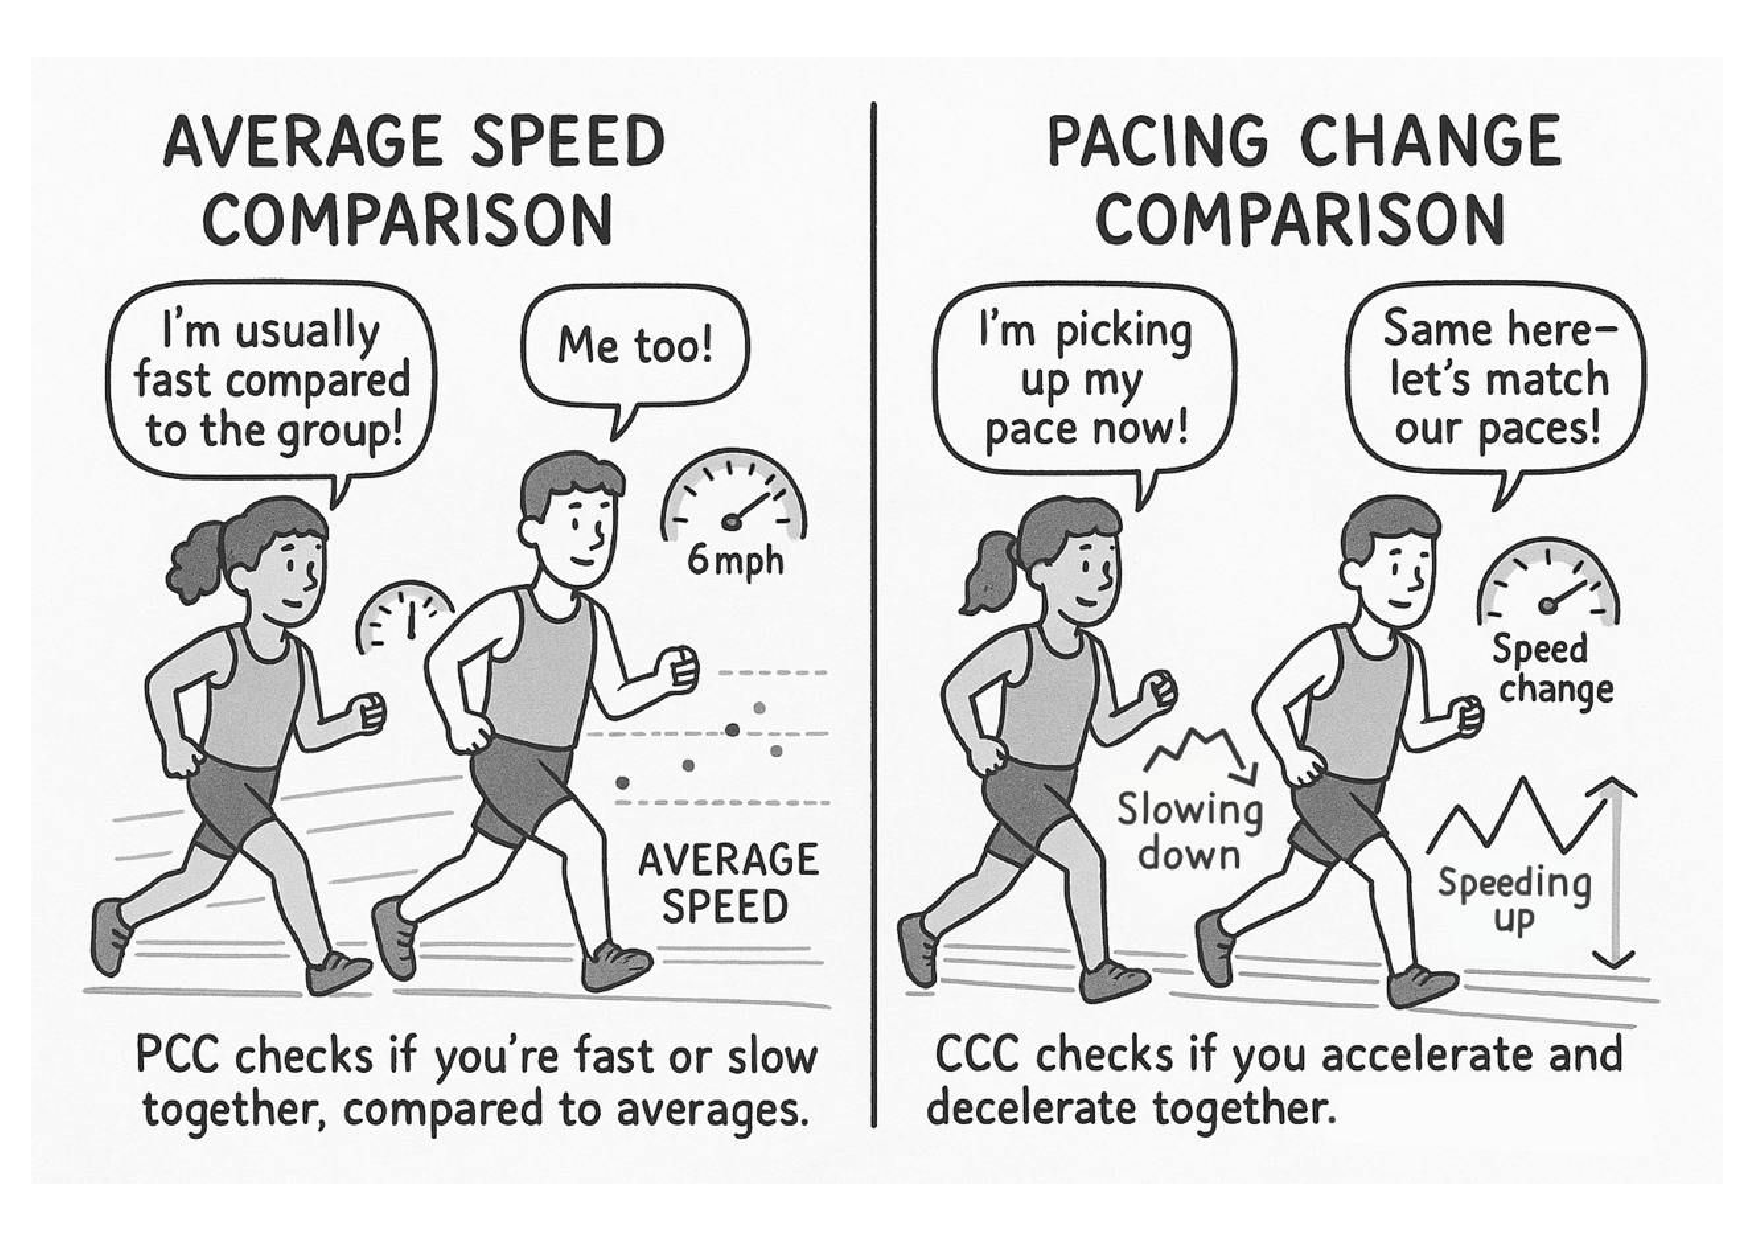
\includegraphics[width=\textwidth]{figure01.pdf}
\caption{Visualization of formula comparison (Increment Based Correlation and Pearson correlation Coefficients) using the running people metaphor} %%%- нужна подпись рисунка
\label{penG}
\end{figure}

For a correct calculation of the $\cic$, the sequences must be presented in an ordered form, reflecting the natural order of observations (e.g., a time series). Prior to calculation, data preprocessing includes handling missing values, removing outliers, and aligning the lengths of the sequences. Subsequently, increments for each index $i$ are computed and substituted into the formula.

The interpretation of results is as follows: values of $\cic$ close to $+1$ indicate a high degree of concordance in the directional changes of the sequences; values close to $-1$ indicate concordance in opposite directions; and values near $0$ suggest the absence of coordinated dynamics. Thus, the $\cic$ provides a means to detect synchrony or asynchrony in the fluctuations between sequences, making it applicable to the analysis of time series, signals, or any datasets where the structure of increments is of primary importance.

Like Pearson correlation this correlation coefficient is also a special case of the Cauchy\allowbreak--\allowbreak Schwarz inequality theorem \cite{r3}:
\begin{enumerate}
\item $\cic$ is based on two vectors in $\mathbb{R}_{n-1}$ space
\[
u = (X_1-X_0, X_2-X_1, \dots, X_n-X_{n-1}), \quad
v = (Y_1-Y_0, Y_2-Y_1, \dots, Y_n-Y_{n-1}).
\]
\item The numerator is the dot product of $u$ and $v$
\[
\langle u,v \rangle = \sum_{i=1}^n (X_i - X_{i-1})(Y_i - Y_{i-1}).
\]
\item The denominator is the product of their Euclidean norms
\[
\|u\| \cdot \|v\| = \sqrt{\sum_{i=1}^n (X_i - X_{i-1})^2} \, \sqrt{\sum_{i=1}^n (Y_i - Y_{i-1})^2}.
\]
\item By the Cauchy–Schwarz inequality, $|\langle u,v \rangle| \le \|u\|\cdot \|v\|$, which gives
\[
-1 \le \frac{\langle u,v \rangle}{\|u\|\cdot \|v\|} \le 1.
\]
\end{enumerate}

As a consequence, $\cic$ possesses the following characteristics:
\begin{itemize}
\item $\cic$ ranges between $-1$ and $1$; it is essentially the cosine of the angle between two normalized centered data vectors.
\item $\cic$ is undefined for constant sequences; the denominator becomes zero.
\item $\cic$ equals $1$ only if forward-difference vectors are positively proportional, and $-1$ if reversed.
\item Unit-free: independent of measurement units, allowing comparison across scales.
\item Symmetric: correlation of $X$ with $Y$ equals correlation of $Y$ with $X$.
\item No linearity assumptions or dependence on averages/peaks.
\item Requires ordered observations (time series, sequences, spatial paths, etc.).
\end{itemize}


\textbf{Note:} The proposed formula differs substantially from the cross-correlation of first differences.

\section{Results}

To validate the applicability of the Cheskidovs’ Correlation Coefficient ($\cic$), several pairs of ordered numerical sequences were analyzed. For demonstration purposes we present here several short simple yet indicative datasets based on functions. We limit the datasets to make the cases more clear, ensuring that results remain the same for the bigger data. We compare it to the well known Pierson coefficient of correlation ($\pcc$) to illustrate the specificity and to show the directions where $\cic$ application could improve data analysis compared to existing approaches.

All data represented ordered series simulating time observations. For each case, both the $\cic$ values and $\pcc$ values were calculated for comparison. For all examples X takes values from $0$ to $8$.


\addExample
  {1}
  {An increasing linear function (with positive slope)}
  {figure11.pdf}
  {0, 1, 2, 3, 4, 5, 6, 7, 8}
  {0, 0.5, 1, 1.5, 2, 2.5, 3, 3.5, 4}
  {1}
  {1}
  {Both coefficients consistently capture the perfect negative dependence. The $\cic$ interprets this as complete synchrony in opposite increments.}



\addExample
  {2}
  {A decreasing linear function (with negative slope)}
  {figure12.pdf}
  {0, 1, 2, 3, 4, 5, 6, 7, 8}
  {4, 3.5, 3,  2.5, 2, 1.5, 1,  0.5, 0}
  {-1}
  {-1}
  {Both coefficients consistently capture the perfect negative dependence. The $\cic$ interprets this as complete synchrony in opposite increments.}


\addExample
  {3}
  {A linear function with increasing and decreasing parts, symmetric}
  {figure13.pdf}
  {0, 1, 2, 3, 4, 5, 6, 7, 8}
  {0, 1, 2, 3, 4, 3, 2, 1, 0}
  {0}
  {0}
  {Both measures indicate the absence of overall directional dependence. The $\cic$ highlights the cancellation of upward and downward increments, producing net synchrony equal to zero.}


\addExample
  {4}
  {A linear function with increasing and decreasing parts, none symmetric (I variant)}
  {figure14.pdf}
  {0, 1, 2, 3, 4, 5, 6, 7, 8}
  {0, 1, 2, 3, 4, 3.5, 3, 2.5, 0}
  {0}
  {0.22}
  {Here, $\pcc$ captures a linear shift around the mean of Y, creating a numerical illusion of correlation with X. $\cic$, on the other hand, is sensitive only to the synchrony of X and Y trends and ultimately returns a correlation value of zero, which aligns with the definition of correlation.} 


\addExample
  {5}
  {A linear function with increasing and decreasing parts, none symmetric (II variant)}
  {figure15.pdf}
  {0, 1, 2, 3, 4, 5, 6, 7, 8}
  {0, 1, 2, 3, 4, 1.5, 1, 0.5, 0}
  {0}
  {-0.17}
  {The negative $\pcc$ reflects a linear shift relative to the mean of Y, thereby producing a spurious indication of correlation. In contrast, the $\cic$ accounts for the directions of change between the variables and therefore yields a correlation value of zero. This result is consistent with the conceptual definition of correlation as a measure of coordinated variation.}


\addExample
  {6}
  {A sinusoid symmetric}
  {figure16.pdf}
  {0, 1, 2, 3, 4, 5, 6, 7, 8}
  {0, 3, 4, 3, 0, -3, -4, -3, 0}
  {0}
  {-0.63}
  {Here $\pcc$ shows a moderately negative relationship due to its linear model constraint, see explanation below. $\cic$ equals zero, reflecting the balance of upward and downward increments across the cycle.}


The Pearson correlation coefficient takes a negative value (\text{$\pcc$} = \text{--}0.63) because it measures the linear association between x and y, not the shape of the relationship.

In this case, x increases steadily from 0 to 8, while y rises and then falls symmetrically around the midpoint. For small x, y tends to be positive (above its mean). For large x - y tends to be negative (below its mean). This creates an overall downward trend — higher y values are associated with smaller x, and lower y values with larger x. Thus, the best-fitting linear regression line slopes downward, leading to a negative correlation.

Even though y is symmetric and nonlinear (roughly sinusoidal), the Pearson coefficient only captures the linear component of that pattern, so the symmetry doesn’t cancel out to zero — it simply produces a moderate negative linear trend.


\addExample
  {7}
  {An inverted sinusoid symmetric}
  {figure17.pdf}
  {0, 1, 2, 3, 4, 5, 6, 7, 8}
  {0, -3, -4, -3, 0, 3, 4, 3, 0}
  {0}
  {0.63}
  {Similar to the previous case, $\pcc$ identifies a moderate correlation. The explanation is the same as for Example 6 with inversion. $\cic$ remains zero, interpreting the balanced cyclic pattern as absence of any synchrony X and Y, which is intuitively visible.}





\begin{table}
\caption{Comparison $\cic$ and $\pcc$}
\label{table1}
\begin{tabular}{@{}lccccl@{}}
\hline
\# &
Type of sequence &
Intuitively &
$\cic$ &
$\pcc$ &
Interpretation \\
\hline
1 & Increasing linear               & 1  & 1 & 1    & Perfect positive dependence \\
2 & Decreasing linear               & -1 & -1 & -1  & Perfect negative dependence \\
3 & Symmetric growth and decline    & 0  & 0 & 0    & No overall dependence \\
 & Non-symmetric growth/decline (I) & 0 & 0 & 0.22 
  & $\pcc$ detects weak correlation,\\
  & & & & & $\cic$ = 0 \\
5 & Non-symmetric growth/decline (II)& 0  & 0 & -0.17 
  & $\pcc$ shows weak negative,\\
  & & & & & $\cic$ = 0 \\
6 & Sinusoid-like, symmetric (I)     & 0  & 0 & -0.63 
  & $\pcc$ shows negative correlation,\\
  & & & & & $\cic$ = 0 \\
7 & Sinusoid-like, symmetric (II)    & 0  & 0 & 0.63 
  & $\pcc$ shows positive correlation,\\
  & & & & & $\cic$ = 0 \\
\hline
\end{tabular}
\end{table}

The comparative analysis demonstrates that the Cheskidovs' Correlation Coefficient ($\cic$) provides stable and interpretable outcomes across a variety of sequence data. In the case of strictly monotonic functions, the values of $\cic$ and the $\pcc$ are equal, confirming that both measures are capable of capturing linear dependencies in a consistent manner.
In contrast, for non-linear or oscillatory patterns, the behavior of $\cic$ differs from that of $\pcc$. For pure examples, $\pcc$ frequently identifies moderate correlations within cyclic none-linear datasets based on deviation of mean values, while $\cic$ systematically converges to zero, reflecting its emphasis on the synchrony of increments (whether they are linear or non-linear nature).

\section{Discussion Section: Interpreting Scientific Research}

Criticism of the Pearson correlation coefficient is not new. For example, in 1921, G. Udny Yule \cite{r1} highlighted issues such as spurious correlation, non-independence of observations, inflated significance, and the dominance of trends, among other limitations. Later, in 1989, Lawrence I-Kuei Lin \cite{r2} emphasized that the Pearson coefficient is insensitive to bias and measures only linear association rather than true agreement. Specifically, it cannot assess whether paired values lie close to the 45$^\circ$ line of perfect concordance, and it may yield inflated values under shifts, making it inadequate for evaluating reproducibility. Sz\'ekely, G. J., Rizzo, M. L., \& Bakirov 1989 \cite{r4} and Chatterjee, S. 2021 \cite{r5} suggested new approaches too. 

The comparative analysis highlights several significant differences between the Cheskidovs' Correlation Coefficient ($\cic$) and traditional correlation measures such as the Pearson correlation coefficient ($\pcc$), Spearman’s rank correlation, and Kendall’s tau. While $\pcc$ reflects linear dependence between variables, and Spearman and Kendall are designed to detect monotonic (not necessarily linear) relationships, $\cic$ is fundamentally distinct in its conceptual approach. It is based on a differential analysis of synchronized increments with a normalized numerator, which captures the direction and concordance of changes within sequences. This focus on global synchrony distinguishes $\cic$ from existing methods and provides an additional methodological perspective.

From a methodological standpoint, $\pcc$ is theoretically valid only under the assumption of linear dependence and approximate normality of the data distribution. In practice, however, $\pcc$ is often applied to nonlinear, unknown or structurally complex datasets. Such usage goes beyond its intended applicability and may lead to misleading or statistically biased interpretations. Spearman’s and Kendall’s coefficients provide greater robustness to nonlinear monotonic transformations but remain sensitive to local ordering of the data rather than global directionality. In contrast, $\cic$ does not have these limitations: it aggregates directional increments across the entire sample, neutralizing local fluctuations that could otherwise generate spurious correlations.

Regarding practical applications, $\cic$ demonstrates clear advantages in situations where the research focus is on the directionality of changes rather than deviations from the mean. For example
\begin{enumerate}
\item Economic time series analysis. In financial markets, stock prices or commodity indices often exhibit oscillatory and cyclical changes. $\pcc$ may detect moderate correlations between assets due to temporary coinciding rises and falls, creating an illusion of dependency. $\cic$ allows identifying true synchrony in changes while ignoring random local fluctuations.

\item Biomedical signal analysis. In physiological data such as heart rate, blood pressure, or EEG signals, cyclical and irregular oscillations are common. $\cic$ can be used to assess synchrony between signals from different organs or brain regions, providing a more accurate reflection of coordinated changes than $\pcc$, which may interpret noisy coincidences as correlations.

\item Environmental and climate studies. Temperature, precipitation, or pollutant concentration data often follow seasonal or wave-like patterns. $\cic$ enables determining the degree to which changes in one variable are synchronized with another without being distorted by temporal oscillations.

\item Technical and engineering systems. For monitoring and predicting the state of complex systems (e.g., vibration sensors in mechanical equipment), it is important to consider the direction of changes rather than absolute values. $\cic$ reliably identifies synchronous behavior of system components, which cannot be achieved using $\pcc$ in cases of nonlinear oscillations.
\end{enumerate}

The novelty of $\cic$ lies in its ability to provide a mathematically consistent and interpretable measure of synchrony for datasets where $\pcc$ and related coefficients may fail. While $\pcc$ is frequently applied to nonlinear or structurally unknown data, potentially producing unreliable conclusions, $\cic$ avoids these pitfalls by not relying on assumptions of linearity or normality. Instead, it directly considers the trend of mutual increments in variables, making it more suitable for analyzing oscillatory, non-monotonic, or non-Gaussian datasets.

Thus, $\cic$ complements existing measures by filling an important methodological gap. It coincides with $\pcc$ in strictly monotonic cases, maintaining comparability, but diverges in oscillatory or complex contexts, avoiding false-positive correlations and providing results that better align with both intuitive and theoretical expectations. This makes $\cic$ a valuable tool for modern data analysis, particularly in dynamic and nonlinear domains where traditional correlation methods exhibit substantial limitations.

While highlighting the advantages of the $\cic$, it is important to note its limitations. The $\cic$ is applicable primarily to ordered time-series data, where the sequential connection is inherent in the nature of the observations. Typical examples include weather records, financial prices, or annual demographic statistics. By contrast, the $\cic$ is not suitable for unordered data such as the heights of students in a classroom, single blood pressure measurements from patients, customer satisfaction scores, IQ test results, or chemical concentrations measured across independent samples. One possible approach in such cases is to impose an order across relevant dimensions before applying the $\cic$.

In special situations where the data exhibit large amplitudes of change and appear incomparable from one step to the next, a logarithmic transformation may be applied, as is common in other mathematical and statistical contexts.

Another approach is to use the Pearson and Cheskidov coefficients of correlation jointly. The former reflects linear interdependence, while the latter is neutral to both linear and nonlinear relationships. The difference between the two measures may provide an indirect indication of the extent of nonlinearity in the correlation structure, which can be valuable in specific applications and large-scale comparative analyses.

\section{Conclusion Section}

This study introduced the Cheskidovs’ Correlation Coefficient ($\cic$) as a novel approach to evaluating synchrony between variables. By applying $\cic$ across monotonic, oscillatory, and mixed time series, the method consistently reflected the presence or absence of directed dependencies. In monotonic cases, $\cic$ reliably reproduces expected correlations, while in more complex forms it maintains stability yielding true negatives (zero correlation) when the condition is indeed false.

Taken together, these findings indicate that $\cic$ functions as a robust and selective measure of synchrony $X$ and $Y$. It reliably identifies perfect monotonic dependencies while avoiding the overestimation of correlation in non-monotonic or oscillatory contexts. These properties suggest that $\cic$ may offer particular utility in the analysis of dynamic datasets of unknown nature, where the directionality of changes carries greater interpretive value than covariance around the means of $X$ and $Y$.

Thus, $\cic$ has proven itself to be a rigorous and complementary tool in correlation analysis, offering clear advantages, although limited to time series cases. For unordered data with no directionality, $\cic$ requires additional data processing and careful consideration of its application.


\begin{thebibliography}{5}
\bibitem{r1}
\textsc{G. Udny Yule} (1921). “On the Time-Correlation Problem, with Especial Reference to the Variate- Difference Correlation Method.” \textit{Journal of the Royal Statistical Society}, Vol. 84, No. 4 (Jul., 1921), pp. 497-537. Published By: Oxford University Press.

\bibitem{r2}
\textsc{Lawrence I-Kuei Lin} (1989). “A Concordance Correlation Coefficient to Evaluate Reproducibility.” \textit{Biometrics}, Vol. 45, No. 1 (Mar., 1989), pp. 255-268.

\bibitem{r3}
\textsc{Cauchy, A.-L.} (1821). "Sur les formules qui résultent de l'emploie du signe et sur > ou <, et sur les moyennes entre plusieurs quantités", \textit{Cours d'Analyse, 1er Partie: Analyse Algébrique} 1821; OEuvres Ser.2 III 373-377.

\bibitem{r4}
\textsc{Székely, G. J., Rizzo, M. L., \& Bakirov, N. K.} (2007). Measuring and Testing Dependence by Correlation of Distances. \textit{Annals of Statistics}, 35(6), pp. 2769–2794.

\bibitem{r5}
\textsc{Chatterjee, S.} (2021). A New Coefficient of Correlation. \textit{Journal of the American Statistical Association}, 116(536), pp. 2009–2022.
\end{thebibliography}


\end{document}
